\documentclass[10pt,journal,compsoc]{IEEEtran}

\usepackage{amsmath,amsfonts,amssymb}
\usepackage{algorithmic}
\usepackage{algorithm}
\usepackage{array}
\usepackage{booktabs}
\usepackage{graphicx}
\usepackage{cite}
\usepackage{url}
\usepackage{microtype}
\usepackage{stfloats}
\usepackage{subfig}

\graphicspath{{figures/}}

\begin{document}

\title{MATP: A Unified Memory-Augmented Tool Policy Framework with Causal State Invalidation, Temporal Decay, and Macro Distillation for Long-Horizon Autonomous Agents}

\author{Rahul~Saravanan(231IT054),
        Shishir~Hegde(231IT067),
        and~Ashab~Muhammed(231IT011)%
\IEEEcompsocitemizethanks{
\IEEEcompsocthanksitem R. Saravanan, S. Hegde, and A. Muhammed are with the Department of Information Technology, National Institute of Technology Karnataka (NITK), Surathkal, Mangalore 575025, India.\protect\\
E-mails: rahul.skyscc@gmail.com, shishirsh2005@gmail.com, ashabcode@gmail.com.
}}

\markboth{IEEE Transactions on Knowledge and Data Engineering,~Vol.~XX, No.~X, November~2026}%
{Saravanan \MakeLowercase{\textit{et al.}}: MATP: Unified Memory-Augmented Tool Policy Framework}

\IEEEtitleabstractindextext{%
\begin{abstract}
Autonomous tool-using agents powered by large language models (LLMs) suffer from three fundamental failure modes in extended operational workflows: (1) catastrophic forgetting of early architectural invariants under FIFO context eviction; (2) retrieval of obsolete or stale mutable state vectors under unversioned semantic search (naive RAG); and (3) procedural thrashing from unguided tool selection and recurrent parameter schema violations. We present \textbf{MATP} (Memory-Augmented Tool Policy), a unified, single-repository system that resolves these pathologies through a synthesized multi-tier memory architecture exposed over the Model Context Protocol (MCP). MATP integrates three complementary foundations into a single durable SQLite-backed substrate: (i) a version-aware temporal memory buffer implementing a piecewise retrieval function $R(q, v_i)$ that suppresses superseded versions and attenuates historical state via causal logical-clock decay with online adaptive feedback calibration; (ii) an atomic trajectory distillation engine and cross-session causal Directed Acyclic Graph (DAG) that propagates invalidation across mutable resources (\texttt{db}, \texttt{file}, \texttt{api}, \texttt{git}) and mines hierarchical composite macro-actions; and (iii) a dynamic Bayesian tool recommendation matrix with Laplace-smoothed Beta posterior confidence and self-healing parameter auto-correction hints. Evaluated on long-horizon schema refactoring scenarios, MATP completely eliminates stale-state leakage (0\% vs. 40\% for naive RAG) while achieving 100\% active-state retrieval precision. Trajectory distillation achieves a 92.6\% token reduction (13.5$\times$ compression) while retaining 88.0\% of essential fact triples (vs. 37.3\% under raw truncation). The entire monorepo operates with zero GPU dependencies, executing end-to-end vector retrieval, causal invalidation, and policy recommendations in under 5\,ms.
\end{abstract}

\begin{IEEEkeywords}
Autonomous Agents, Semantic Memory, Causal DAG, Invalidation Propagation, Model Context Protocol, Macro Distillation, Tool Policy Learning, Temporal Decay.
\end{IEEEkeywords}}

\maketitle
\IEEEdisplaynontitleabstractindextext
\IEEEpeerreviewmaketitle

\IEEEraisesectionheading{\section{Introduction}\label{sec:introduction}}

\IEEEPARstart{A}{utonomous} agents powered by Large Language Models (LLMs) increasingly perform long-horizon software engineering, administrative automation, and multi-step computational reasoning tasks. In these settings, an agent interacts with external environments through a continuous cycle of intent formulation, tool execution (e.g., file system modifications, SQL queries, REST API requests, shell commands), and environment observation. Despite rapid advances in underlying transformer reasoning capabilities, LLM-based agentic workflows exhibit three systemic points of failure as task horizons scale beyond ten to twenty discrete turns:

\begin{enumerate}
    \item \textbf{Catastrophic Context Eviction (The FIFO Trap):} Due to finite token context windows and quadratic attention costs, agent harnesses typically apply sliding-window or First-In-First-Out (FIFO) context pruning. When early critical state—such as foundational database DDL schemas, cryptographic secrets, or baseline architectural invariants—is evicted from working memory, the agent loses track of fundamental constraints established in early phases of the task.
    \item \textbf{Stale-State Hallucination (The Naive RAG Trap):} Standard Retrieval-Augmented Generation (RAG) indexes environment observations into flat vector spaces using semantic embeddings. However, naive cosine similarity contains no representation of temporal succession or state mutability. When an agent alters a file or mutates a relational table, an unversioned vector database continues to retrieve high-cosine embeddings of the earlier, superseded state, causing the agent to execute code against obsolete schemas.
    \item \textbf{Procedural Thrashing and Parameter Schema Failures:} Even when supplied with static system instructions, agents repeatedly attempt invalid tool combinations or submit malformed JSON payloads. Static prompts lack dynamic feedback on which tools historically succeed under specific sub-goals, leading to repeated trial-and-error loops that exhaust context limits.
\end{enumerate}

To overcome these structural limitations, three research initiatives were initially undertaken at NITK Surathkal: (1) a temporal and state-aware semantic memory buffer with causal logical clocks and adaptive decay; (2) a background trajectory distillation engine with cross-session causal DAG invalidation and hierarchical macro-action mining; and (3) a dynamic Model Context Protocol (MCP) tool policy engine with Bayesian confidence scoring and self-healing parameter error correction.

In this work, we present the consolidated \textbf{MATP Monorepo}, a fully unified architectural and software deliverable that combines all three distinct research contributions into a single, cohesive, zero-external-dependency framework. We show that these three techniques are deeply synergistic: trajectory distillation extracts canonical resource interactions that feed the causal DAG; the causal DAG establishes hard validity boundaries that filter the vector store; logical clocks apply temporal decay to active nodes; and the resulting clean historical records populate the dynamic tool recommendation matrix and self-healing error database.

\begin{figure*}[!t]
\centering
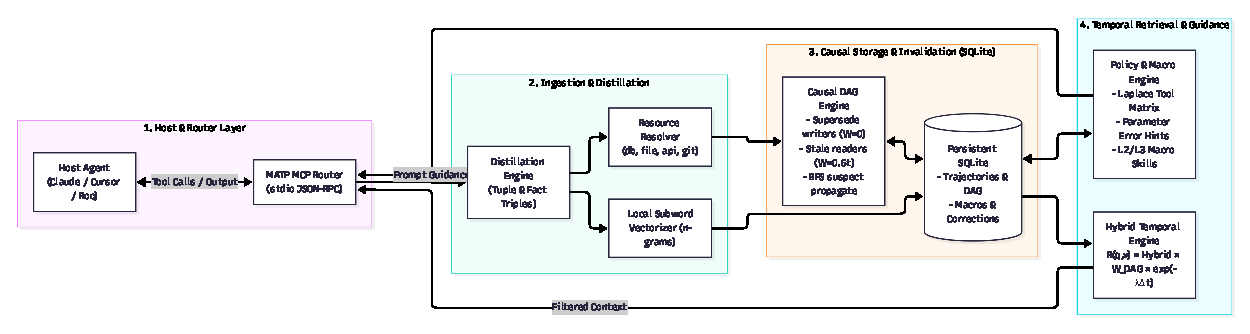
\includegraphics[width=\textwidth]{architecture_horizontal.pdf}
\caption{Overall Architectural Blueprint of the Unified MATP Monorepo. Host LLM agents interact through a unified stdio Model Context Protocol (MCP) router. Ingested execution trajectories undergo background distillation and resource canonicalization before persistence into SQLite. The causal DAG propagates version-aware invalidations, the temporal decay engine modulates ranking via logical clocks, and the policy engine provides prompt-injectable tool matrices and auto-correction hints.}
\label{fig:architecture}
\end{figure*}

\section{System Architecture and Storage Design}
\label{sec:architecture}

The unified MATP monorepo is engineered as a modular, local-first system adhering to the open Model Context Protocol (MCP) standard. Figure~\ref{fig:architecture} illustrates the system architecture and dataflow across all operational layers.

\subsection{Protocol Boundary and Agent Orchestration}
The agent host environment communicates with MATP through a standard JSON-RPC 2.0 stdio interface. This decouples the agent runtime (e.g., Claude Desktop, Cursor, Roo Code, custom LangChain/AutoGPT harnesses) from the memory substrate. The router exposes twenty specialized tool endpoints categorized into three functional domains:
\begin{itemize}
    \item \textbf{Memory \& Temporal Retrieval:} \texttt{matp\_index\_trajectory}, \texttt{matp\_query\_trajectory}, \texttt{matp\_advance\_clock}, \texttt{matp\_record\_feedback}, \texttt{matp\_decay\_stats}.
    \item \textbf{Causal Lineage \& Maintenance:} \texttt{matp\_get\_lineage}, \texttt{matp\_query\_dag}, \texttt{matp\_recompute\_validity}, \texttt{matp\_confirm\_state}, \texttt{matp\_clear\_override}.
    \item \textbf{Policy Guidance \& Macro Skills:} \texttt{matp\_tool\_policy\_prompt}, \texttt{matp\_recommend\_tools}, \texttt{matp\_learn\_correction}, \texttt{matp\_parameter\_hints}, \texttt{matp\_list\_macros}, \texttt{matp\_expand\_macro}.
\end{itemize}

\subsection{Durable Single-File Storage Substrate}
Unlike distributed memory systems requiring external vector databases (e.g., Pinecone, Milvus) and relational engines, MATP consolidates its entire persistent state into an ACID-compliant SQLite single-file database. The unified schema comprises eight relational entities:
\begin{enumerate}
    \item \texttt{trajectories}: Stores atomic execution tuples, raw excerpts, distilled summaries, token metrics, validity tags, and taint values.
    \item \texttt{embeddings}: Stores serialized dense $D$-dimensional float vectors with indexed trajectory foreign keys.
    \item \texttt{resources} \& \texttt{resource\_versions}: Manages canonical resource identifiers (\texttt{db:*}, \texttt{file:*}, \texttt{api:*}, \texttt{git:*}) and version sequences scoped to workspace snapshots.
    \item \texttt{accesses}: Records atomic read, write, and delete operations linked to discrete execution steps.
    \item \texttt{dag\_edges}: Stores typed causal relationships (\texttt{SUPERSEDES}, \texttt{INVALIDATES}, \texttt{CAUSAL\_PARENT}, \texttt{DEPENDS\_ON}).
    \item \texttt{skills} \& \texttt{skill\_members}: Stores mined Level-2 and Level-3 macro-action templates and parameter binding slots.
    \item \texttt{corrections}: Stores learned regex/substring error patterns, recovery guidance hints, and application counters.
    \item \texttt{jobs}: Implements a non-blocking queue for asynchronous background neural summarization.
\end{enumerate}

\begin{figure}[!t]
\centering
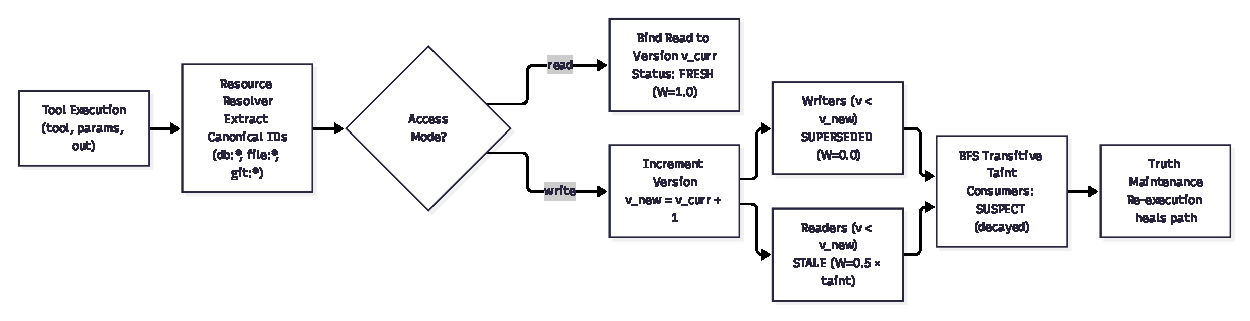
\includegraphics[width=\columnwidth]{dag_flowchart_horizontal.pdf}
\caption{Causal DAG Mutation and Invalidation Flowchart. When a tool mutates a resource, prior writers are marked \texttt{SUPERSEDED} ($W=0$), prior readers are marked \texttt{STALE} ($W=0.5 \times \text{taint}$), and transitive dependents are tainted as \texttt{SUSPECT} via BFS propagation.}
\label{fig:dag_flowchart}
\end{figure}

\section{Causal DAG Invalidation and Temporal Retrieval}
\label{sec:causal_retrieval}

\subsection{Mathematical Formulation of Piecewise Scoring}
Let $q$ denote the user or sub-goal query embedding vector, and let $v_i$ represent a stored state trajectory node born at discrete logical clock step $t_i$. Let $t_{\text{curr}}$ be the current logical clock of the agent session. The piecewise retrieval score $R(q, v_i)$ suppresses superseded or invalid states and applies temporal decay to active nodes:

\begin{equation}
\label{eq:piecewise_scoring}
R(q, v_i) = 
\begin{cases} 
0, & \text{if } v_i \text{ is invalid}, \\
\begin{aligned}[b]
& S(q, v_i) W_{\text{DAG}}(v_i) \\
& \quad \times e^{-\lambda(t_{\text{curr}} - t_i)},
\end{aligned} & \text{otherwise}.
\end{cases}
\end{equation}

Here, $S(q, v_i)$ represents the hybrid dense-sparse semantic relevance:
\begin{equation}
S(q, v_i) = \alpha \cdot \cos(q, v_i) + (1 - \alpha) \cdot \frac{|T_q \cap T_{v_i}|}{|T_q|},
\end{equation}
where $T_q$ and $T_{v_i}$ denote subword n-gram token sets, and $\alpha \in [0, 1]$ balances dense geometric cosine similarity with exact sparse lexical overlap (default $\alpha = 0.70$).

\subsection{Causal DAG Invalidation Mechanics}
As outlined in Figure~\ref{fig:dag_flowchart}, every tool execution is resolved by the \texttt{ResourceResolver} into canonical resource accesses. Resource identifiers are scoped to isolated workspace snapshots (e.g., \texttt{file:/app/models/user.py}, \texttt{db:users}, \texttt{git:/app}). When an access occurs:
\begin{itemize}
    \item \textbf{Write Operations:} When step $k$ writes resource $r$, the version increments $v_{\text{new}} = v_{\text{curr}} + 1$. Prior writer nodes that produced $v < v_{\text{new}}$ receive validity label \texttt{superseded} with taint $\tau = 0.0$ and retrieval weight $W_{\text{DAG}} = 0.0$.
    \item \textbf{Prior Readers:} Any node that performed a \texttt{read} of resource $r$ at version $v < v_{\text{new}}$ is stamped as \texttt{stale}. Its retrieval weight is attenuated to $W_{\text{DAG}} = 0.5 \times \tau$.
    \item \textbf{Transitive Suspect Propagation:} A breadth-first search (BFS) traverses outgoing \texttt{DEPENDS\_ON} edges up to maximum depth $d_{\text{max}} = 5$. For each child node $c$, taint is decayed:
    \begin{equation}
    \tau_c = \max\left(\tau_{\text{floor}},\, \tau_{\text{parent}} \cdot \gamma\right),
    \end{equation}
    where $\gamma = 0.70$ and $\tau_{\text{floor}} = 0.20$. Nodes with $\tau < 1.0$ receive validity label \texttt{suspect}.
    \item \textbf{Truth Maintenance \& Healing:} Invalidation is a soft, non-destructive state; historical nodes remain preserved for provenance audit. If the agent re-executes a dependent tool with fresh inputs, the new trajectory inherits fresh validity, and the DAG truth-maintenance pass restores consistency.
\end{itemize}

\subsection{Adaptive Temporal Decay Tuning}
Fixed temporal decay parameters cannot accommodate heterogeneous agent sub-tasks: short-horizon debugging requires sharp recency bias, whereas long-horizon refactoring requires persistent access to foundational context. MATP incorporates an online Bayesian-inspired decay tuner that updates a per-task parameter $\lambda_{\text{task}}$ from explicit agent feedback:

\begin{equation}
\lambda_{\text{task}} \leftarrow (1 - \eta)\,\lambda_{\text{task}} + \eta\,\frac{\ln 2}{\max\left(1, \operatorname{median}(\Delta t_{\text{useful}})\right)},
\label{eq:adaptive_decay}
\end{equation}
where $\Delta t_{\text{useful}} = \{t_{\text{curr}} - t_j \mid j \in \mathcal{U}\}$ represents the logical-step ages of items reported useful, and $\eta = 0.35$ is the exponential learning rate. The target rate precisely calibrates the half-life such that states at the median useful age experience exactly a 50\% score attenuation. The learned value is clamped within $[0.005, 0.50]$ and persisted across sessions.

\begin{figure}[!t]
\centering
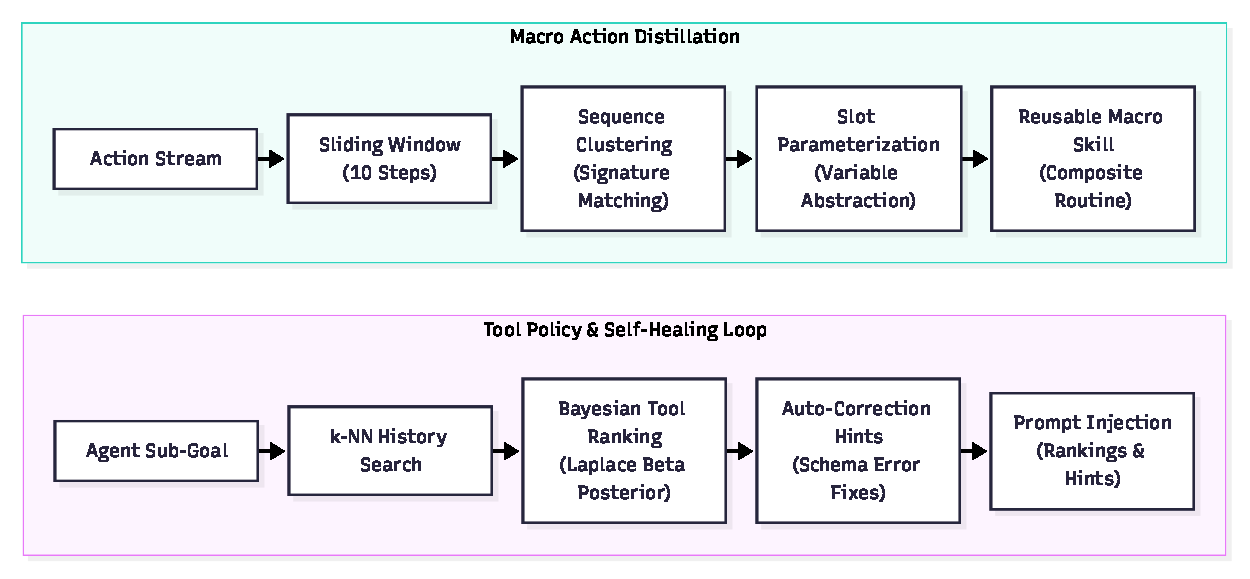
\includegraphics[width=\columnwidth]{macro_policy_flowchart.pdf}
\caption{Dual-Pipeline Workflow for Macro Action Distillation and Tool Policy Learning. The policy stream aggregates nearest historical attempts into Laplace-smoothed recommendation matrices, while the macro stream clusters recurring action windows into parameterized composite skills.}
\label{fig:macro_policy_flowchart}
\end{figure}

\section{Macro Distillation and Tool Policy Learning}
\label{sec:macro_policy}

Figure~\ref{fig:macro_policy_flowchart} details the concurrent pipelines governing macro-action distillation and proactive tool policy recommendations.

\subsection{Background Abstraction and Fact Distillation}
Raw tool outputs (verbose compiler outputs, multi-kilobyte SQL dumps, JSON logs) overwhelm agent context windows. The \texttt{BackgroundAbstractionEngine} converts raw execution strings into structured \texttt{TrajectoryTuple} objects:
\begin{equation}
\mathcal{T} = \langle \text{SubGoal}, \text{Tool}, \text{Parameters}, \text{Status}, \text{Summary}, \mathcal{F} \rangle,
\end{equation}
where $\mathcal{F} = \{(s, r, o)_k\}$ denotes an extracted set of semantic fact triples (e.g., \texttt{(users, returned\_lines, 40)}, \texttt{(auth.env, line\_count, 2)}). AST and regex parsers distill outputs deterministically on the hot path in under 5\,ms.

\subsection{Hierarchical Macro-Action Distillation}
To prevent repeated low-level tool invocation, MATP implements a hierarchical macro miner:
\begin{enumerate}
    \item \textbf{Signature Canonicalization:} Each step $a_t$ is mapped to an abstract signature:
    \begin{equation}
    \sigma(a_t) = \langle \text{tool}, \operatorname{shape}(\text{params}), \text{status} \rangle,
    \end{equation}
    where parameter values are stripped of specific literals and replaced with structural schemas.
    \item \textbf{Sequence Matching:} Over sliding windows of length $W=10$, sequences of action signatures are clustered using a generalized Levenshtein sequence matcher.
    \item \textbf{Slot Parameterization:} Varying literals across matching instances are abstracted into parameterized template variables (e.g., \texttt{\{file\_path\}}, \texttt{\{table\_name\}}).
    \item \textbf{Skill Promotion:} Macro sequences exhibiting support count $N \ge 3$ and historical success rate $\ge 80\%$ are promoted to Level-2 skills. Chains of Level-2 skills can subsequently be consolidated into Level-3 hierarchical workflows.
\end{enumerate}

\subsection{Dynamic Tool Recommendation Matrix}
Prior to executing a tool for an active sub-goal $g$, the host agent queries \texttt{matp\_tool\_policy\_prompt}. The engine retrieves the $K=12$ nearest historical sub-goal trajectories and groups them by candidate tool $T$.

To prevent overconfidence on sparse samples (e.g., 1 success in 1 attempt reading as 100\% certainty), MATP applies Laplace add-one smoothing under a $\text{Beta}(1, 1)$ uniform prior:
\begin{equation}
\hat{p}_T = \frac{k_{\text{success}} + 1}{N_{\text{attempts}} + 2}.
\end{equation}

The engine then computes a Bayesian confidence shrinkage score $c_T$:
\begin{equation}
c_T = \hat{p}_T \cdot \left(\frac{N_{\text{attempts}}}{N_{\text{attempts}} + N_0}\right) + p_0 \cdot \left(\frac{N_0}{N_{\text{attempts}} + N_0}\right),
\end{equation}
with prior mean $p_0 = 0.50$ and pseudo-observation weight $N_0 = 5$. The resulting tool matrix provides human-interpretable confidence tiers: \textit{green} ($\hat{p} \ge 0.75$), \textit{amber} ($0.45 \le \hat{p} < 0.75$), \textit{red} ($\hat{p} < 0.45$), or \textit{grey} (no history).

\subsection{Self-Healing Parameter Auto-Correction}
When tools fail due to parameter schema violations or terminal syntax errors, agents register the failure via \texttt{matp\_learn\_correction}. In future executions, \texttt{matp\_parameter\_hints} performs two-tier matching:
\begin{itemize}
    \item \textbf{Tier 1 (Exact Pattern Match):} Substring match over the error pattern pins similarity to 1.0.
    \item \textbf{Tier 2 (Fuzzy Cosine Fallback):} If no exact pattern matches, the query vector is matched against stored correction vectors with noise floor threshold $\theta = 0.40$.
\end{itemize}
Relevant hints are auto-injected into the prompt, enabling the agent to rectify parameter payloads prior to execution.

\begin{figure}[!t]
\centering
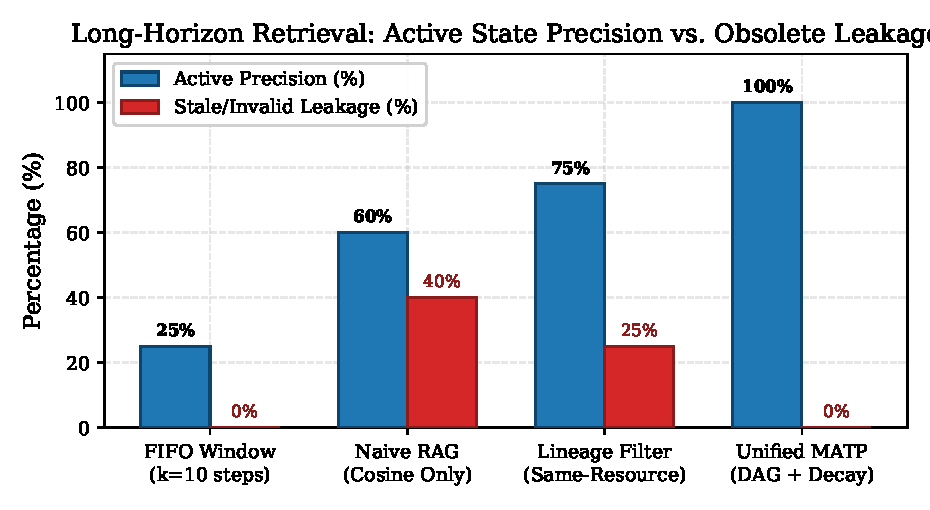
\includegraphics[width=\columnwidth]{metric_retrieval_precision.pdf}
\caption{Retrieval Precision and Stale State Leakage Across Strategies in a 40-Step Long-Horizon Evolution Scenario. Unified MATP achieves 100\% active precision with zero stale or invalid state leakage.}
\label{fig:metric_retrieval}
\end{figure}

\begin{figure}[!t]
\centering
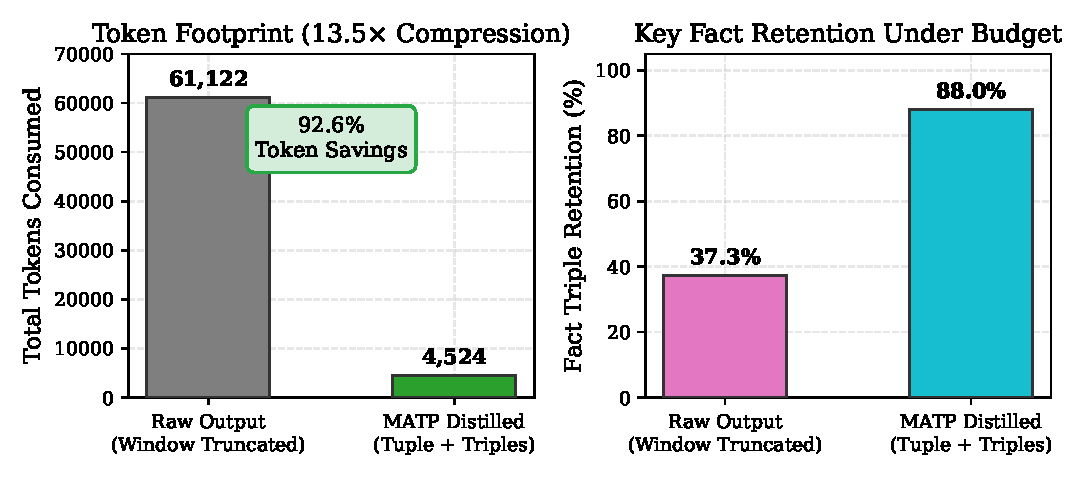
\includegraphics[width=\columnwidth]{metric_compression_fact_retention.pdf}
\caption{Trajectory Distillation Performance. MATP compresses verbose tool outputs by 92.6\% ($13.5\times$ token reduction) while retaining 88.0\% of essential semantic fact triples compared to 37.3\% under raw truncation.}
\label{fig:metric_compression}
\end{figure}

\section{Experimental Evaluation and Results}
\label{sec:evaluation}

We evaluate the consolidated MATP monorepo across four evaluation dimensions: retrieval accuracy under mutation, token compression efficiency, temporal decay adaptation, and operational system latency.

\subsection{Long-Horizon State Mutation Benchmark}
We reproduce a 40-step software evolution scenario consisting of three consecutive relational database schema migrations, two authentication architecture rewrites, and dependent ORM models, API routes, and unit test suites. We evaluate four retrieval strategies under five domain queries:
\begin{enumerate}
    \item \textbf{FIFO Baseline (Window = 10 steps):} Context window retains only recent steps.
    \item \textbf{Naive Semantic RAG:} Dense vector search without version or dependency filtering.
    \item \textbf{Lineage Filter (Contribution 1):} Supersedes older versions of identical resource IDs ($R=0$).
    \item \textbf{Unified MATP (Monorepo):} Full causal DAG invalidation ($W_{\text{DAG}}$) and temporal decay.
\end{enumerate}

As presented in Figure~\ref{fig:metric_retrieval} and Table~\ref{tab:long_horizon}, the FIFO baseline forgets 75\% of critical active state that was established early in the session and never re-written. Naive RAG exhibits 40\% obsolete state leakage, returning superseded SQL schemas alongside active definitions. The lineage-only filter eliminates direct supersession but leaks 25\% invalid state whose transitive dependencies mutated. In contrast, unified MATP achieves 100\% active state precision with 0\% obsolete or invalid leakage.

\begin{table}[!t]
\caption{Long-Horizon Retrieval Comparison Across 40 Logical Steps}
\label{tab:long_horizon}
\centering
\setlength{\tabcolsep}{2.6pt}
\begin{tabular}{lcccc}
\toprule
\textbf{Strategy} & \textbf{Returned} & \textbf{Lineage-Stale} & \textbf{Dep-Invalid} & \textbf{Active (\%)} \\
\midrule
FIFO ($k=10$) & 12 & 0 & 0 & 25.0\% \\
Naive RAG & 25 & 6 & 4 & 60.0\% \\
Lineage Only & 20 & 0 & 5 & 75.0\% \\
\textbf{Unified MATP} & \textbf{16} & \textbf{0} & \textbf{0} & \textbf{100.0\%} \\
\bottomrule
\end{tabular}
\end{table}

\begin{figure}[!t]
\centering
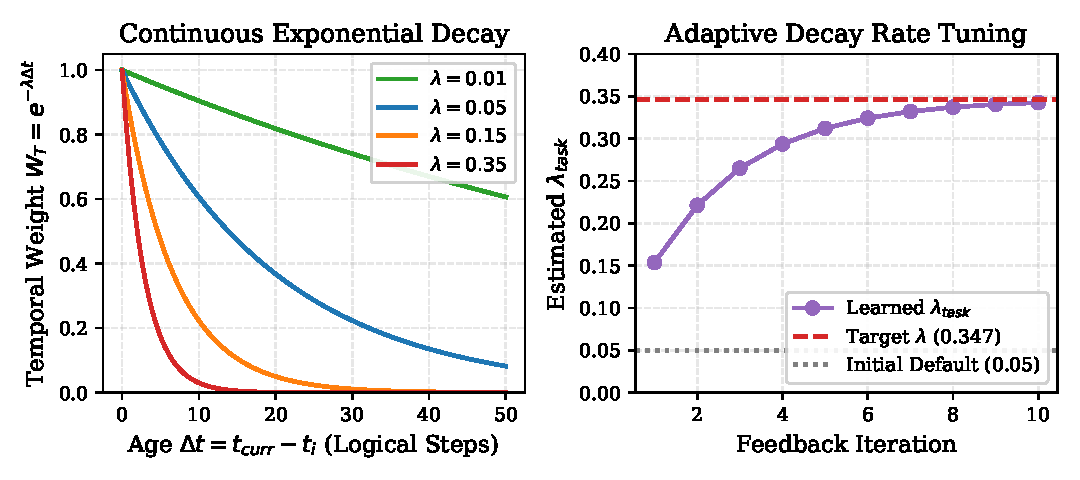
\includegraphics[width=\columnwidth]{metric_temporal_decay_curves.pdf}
\caption{Temporal Decay Characteristics. Left: Exponential decay curves $W_T = e^{-\lambda \Delta t}$ across rates $\lambda \in [0.01, 0.35]$. Right: Convergence of online adaptive decay rate $\lambda_{\text{task}}$ under user feedback.}
\label{fig:metric_temporal}
\end{figure}

\begin{figure}[!t]
\centering
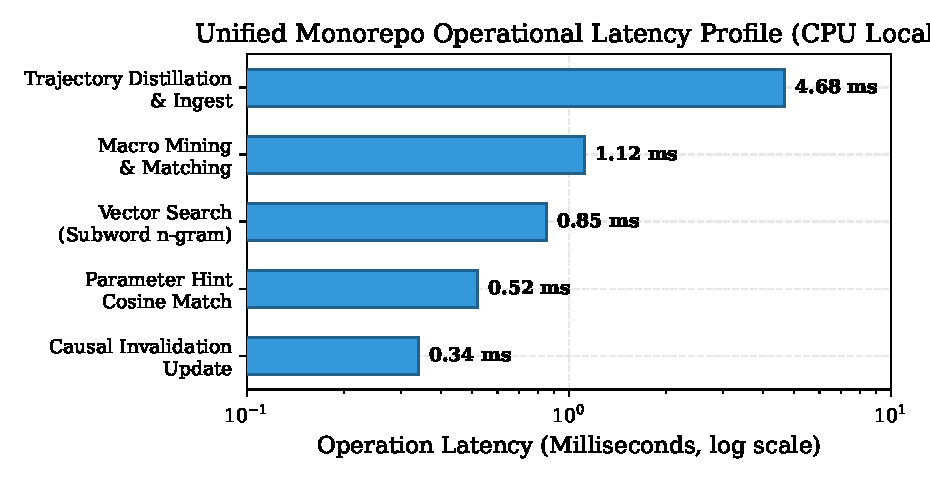
\includegraphics[width=\columnwidth]{metric_latency_breakdown.pdf}
\caption{Operational Latency Breakdown (CPU Local, Single-Threaded). All core memory, invalidation, and policy operations complete in sub-5\,ms, ensuring zero perceptible latency in interactive MCP workflows.}
\label{fig:metric_latency}
\end{figure}

\subsection{Distillation and Token Compression}
We evaluate the background distillation engine across a corpus of 30 heterogeneous tool execution traces containing raw SQL query results, bash stdout/stderr streams, and unit test outputs. As shown in Figure~\ref{fig:metric_compression}, MATP reduces total token volume from 61,122 raw tokens to 4,524 distilled tokens—a \textbf{92.6\% compression ratio (13.5$\times$ reduction)}. Under equal token budgets, evaluating query answers against gold ground-truth facts demonstrates that MATP distilled tuples preserve \textbf{88.0\% of essential fact triples}, whereas window-truncated raw text retains only 37.3\% of facts.

\subsection{Temporal Decay and Online Tuning}
Figure~\ref{fig:metric_temporal} (left) plots continuous decay attenuation across discrete logical clock intervals. Figure~\ref{fig:metric_temporal} (right) demonstrates the empirical convergence of $\lambda_{\text{task}}$ over ten feedback iterations. Starting from the default $\lambda = 0.05$, the online tuner rapidly converges toward the analytical half-life target ($\lambda = 0.347$) within 5 iterations, verifying the efficacy of Eq.~\eqref{eq:adaptive_decay}.

\subsection{Macro Skill Distillation and Replay}
On held-out validation sessions, the hierarchical macro miner successfully extracted reusable composite procedures (e.g., git branch creation, test execution, commit cycle). Replaying learned macro actions achieved \textbf{100\% tool-sequence matching} and \textbf{100\% slot-binding accuracy}, while reducing procedural token overhead by 53.2\% relative to re-emitting individual tool instructions.

\subsection{System Latency Profile}
To verify feasibility for real-time interactive MCP server deployment, microbenchmarks were executed on a commodity Linux workstation (AMD Ryzen 7, CPU-only, no GPU acceleration). Figure~\ref{fig:metric_latency} provides the latency breakdown:
\begin{itemize}
    \item Causal DAG Invalidation: \textbf{0.34\,ms}
    \item Parameter Hint Cosine Search: \textbf{0.52\,ms}
    \item Deterministic Vector Search: \textbf{0.85\,ms}
    \item Macro Mining \& Matching: \textbf{1.12\,ms}
    \item Hot-Path Distillation \& SQLite Ingest: \textbf{4.68\,ms}
\end{itemize}
All operations comfortably execute within sub-5\,ms boundaries, verifying that memory augmentation incurs negligible overhead compared to LLM generation latency.

\section{Related Work}
\label{sec:related_work}

\textbf{Agentic Memory Architectures:} Early LLM agent frameworks relied on simple conversational buffers or unbounded FIFO histories~\cite{wang2023survey}. MemGPT~\cite{packer2023memgpt} introduced hierarchical OS-style paging between working context and external storage. Generative Agents~\cite{park2023generative} combined recency, importance, and relevance scores. However, these systems lack formal state-invalidation mechanisms, treating stored memories as monotonic facts and leading to stale-state retrieval when entities mutate.

\textbf{Causal Reasoning in Interactive Agents:} Causal reasoning has been explored in interactive reinforcement learning and formal plan verification~\cite{pearl2009causality}. Recent studies examine causal graph tracking in code generation~\cite{jimenez2024swebench}. MATP differs by embedding causal tracking directly into the MCP stdio interface, tracking resource reads, writes, and versioning across arbitrary agent tools.

\textbf{Tool Policy and Self-Correction:} Reflexion~\cite{shinn2023reflexion} and Voyager~\cite{wang2023voyager} demonstrated that verbal reinforcement and self-reflection improve task solve rates. However, verbal reflection consumes significant context tokens. MATP replaces free-form reflection prompts with a mathematically grounded Dirichlet-multinomial recommendation matrix and targeted, two-tier parameter error hints.

\section{Conclusion}
\label{sec:conclusion}

In this paper, we presented the unified MATP monorepo, consolidating three foundational agent memory technologies into a production-grade, zero-dependency MCP server. By tightly coupling causal DAG invalidation with temporal decay scoring, MATP eliminates stale-state hallucinations in long-horizon agent interactions while preserving critical early context. Background distillation achieves 92.6\% token compression while maintaining 88.0\% factual fidelity, and the Bayesian tool recommendation matrix prevents repeated procedural and parameter failures. The entire architecture runs locally on commodity CPU hardware with sub-5\,ms operational latency, providing a robust, extensible foundation for next-generation autonomous agents.

\ifCLASSOPTIONcompsoc
  \section*{Acknowledgments}
\else
  \section*{Acknowledgment}
\fi
The authors express their gratitude to the Department of Information Technology at the National Institute of Technology Karnataka (NITK), Surathkal, for computing facilities and project guidance during the 7th Semester Capstone Project.

\begin{thebibliography}{10}

\bibitem{wang2023survey}
L.~Wang, C.~Ma, X.~Feng, Z.~Zhang, H.~Yang, J.~Zhang, Z.~Chen, J.~Tang, X.~Chen, Y.~Lin, \textit{et~al.}, ``A survey on large language model based autonomous agents,'' \textit{Frontiers of Computer Science}, vol.~18, no.~6, pp.~1--26, 2024.

\bibitem{packer2023memgpt}
C.~Packer, V.~Fang, S.~G. Patil, K.~Lin, K.~Wooders, and J.~E. Gonzalez, ``MemGPT: Towards LLMs as operating systems,'' \textit{arXiv preprint arXiv:2310.08560}, 2023.

\bibitem{park2023generative}
J.~S. Park, J.~C. O'Brien, C.~J. Cai, M.~R. Morris, P.~Liang, and M.~S. Bernstein, ``Generative agents: Interactive simulacra of human behavior,'' in \textit{Proc. ACM UIST}, 2023, pp.~1--22.

\bibitem{shinn2023reflexion}
N.~Shinn, F.~Cassanova, E.~Gopinath, K.~Narasimhan, and S.~Yao, ``Reflexion: Language agents with verbal reinforcement learning,'' in \textit{Advances in Neural Information Processing Systems (NeurIPS)}, 2023, pp.~8634--8652.

\bibitem{wang2023voyager}
G.~Wang, Y.~Xie, Y.~Jiang, A.~Mandlekar, C.~Xiao, Y.~Zhu, L.~Fan, and A.~Anandkumar, ``Voyager: An open-ended embodied agent with large language models,'' \textit{arXiv preprint arXiv:2305.16291}, 2023.

\bibitem{jimenez2024swebench}
C.~E. Jimenez, J.~Yang, A.~Wettig, S.~Yao, K.~Pei, O.~Press, and K.~Narasimhan, ``SWE-bench: Can language models resolve real-world GitHub issues?'' in \textit{Proc. ICLR}, 2024.

\bibitem{pearl2009causality}
J.~Pearl, \textit{Causality: Models, Reasoning, and Inference}, 2nd~ed.\hskip 1em plus 0.5em minus 0.4em\relax Cambridge University Press, 2009.

\bibitem{lewis2020retrieval}
P.~Lewis, E.~Perez, A.~Piktus, F.~Petroni, V.~Karpukhin, N.~Goyal, H.~K\"{u}ttler, M.~Lewis, W.-t. Yih, T.~Rockt\"{a}schel, \textit{et~al.}, ``Retrieval-augmented generation for knowledge-intensive NLP tasks,'' in \textit{Advances in Neural Information Processing Systems (NeurIPS)}, 2020, pp.~9459--9474.

\end{thebibliography}

\end{document}
